\documentclass[11pt,a4paper]{article}
\usepackage[utf8]{inputenc}
\usepackage[margin=2.0cm]{geometry}
\usepackage{amsmath,amssymb}
\usepackage{graphicx}
\usepackage{booktabs}
\usepackage{hyperref}
\usepackage{fancyhdr}
\usepackage{microtype}

\setlength{\headheight}{14pt}

\hypersetup{
    colorlinks=true,
    linkcolor=blue,
    citecolor=blue,
    urlcolor=blue,
    pdftitle={First-Order Explosive Synchronization via Markov-Blanket Boundary Gating in Modular Oscillator Networks},
    pdfauthor={Bruno Lucardo Olivaes}
}

\pagestyle{fancy}
\fancyhf{}
\rhead{Explosive Synchronization via Markov-Blanket Gating}
\lhead{Olivaes (2026)}
\cfoot{\thepage}

\title{\textbf{First-Order Explosive Synchronization via Markov-Blanket Boundary Gating in Modular Oscillator Networks}}

\author{
    \textbf{Bruno Lu\c{c}ardo Olivaes}\\
    \small Independent Researcher, Rio de Janeiro, Brazil\\
    \small ORCID: \href{https://orcid.org/0009-0003-5351-446X}{0009-0003-5351-446X} \quad $\vert$ \quad Email: \href{mailto:brunoolivaes@gmail.com}{brunoolivaes@gmail.com}
}

\date{November 2026}

\begin{document}

\maketitle

\begin{abstract}
In networked dynamical systems, the classical Kuramoto transition to macroscopic collective synchronization is universally characterized as a continuous, second-order phase transition governed by a supercritical pitchfork bifurcation ($R \propto (K - K_c)^\beta$). Here, we demonstrate that partitioning oscillator networks into distinct topological modules separated by Markov blankets---in strict accordance with the Active Inference precision-weighting formulation of the Free Energy Principle (FEP)---fundamentally alters the universality class of the phase transition. When modular coupling strength is dynamically gated by joint cross-blanket boundary consensus ($\mathcal{G}(t) = [R_{\mathcal{B}}^{\mathrm{joint}}(t)]^\gamma$, $\gamma = 2.40$), subcritical phase locking is suppressed below a critical threshold $K_c^{\mathrm{fwd}} = 3.50$. Exceeding threshold triggers cooperative blanket-mediated feedback, inducing an abrupt, discontinuous first-order explosive jump ($\Delta R = 0.7335$) accompanied by a wide bistable hysteresis loop extending down to $K_c^{\mathrm{bwd}} = 1.50$ ($\Delta K_{\mathrm{hyst}} = 2.00$, directional hysteresis area $\mathcal{A}_{\mathrm{hyst}} = 1.4932$, vs.\ $\mathcal{A}_{\mathrm{hyst}} = 0.0101$ on the identical ungated reference $\mathcal{G} \equiv 1$). Consistent with global $U(1)$ phase-rotation invariance, we reconstruct the subcritical sixth-order Landau-Ginzburg effective free energy $\mathcal{F}(R; K) = \frac{1}{2} a_0 (K_c - K) R^2 - \frac{1}{4} b R^4 + \frac{1}{6} c R^6$, proving how a negative quartic coefficient ($b > 0$) stabilized by sextic saturation ($c > 0$) sustains metastable coexistence. Joint forward--backward Bayesian Information Criterion (BIC) model selection delivers decisive statistical evidence ($\Delta\mathrm{BIC} = +267.53$) favoring the first-order spinodal model over a continuous saturating pitchfork, while correctly preferring the second-order continuous branch ($\Delta\mathrm{BIC} = -153.30$) on the ungated reference. These results establish a rigorous statistical-mechanics bridge between Active Inference boundaries, metastability, and explosive network transitions.
\end{abstract}

\vspace{0.45cm}
\noindent\textbf{Keywords:} Explosive Synchronization, Kuramoto Model, Markov Blankets, Free Energy Principle, Active Inference, Subcritical Landau-Ginzburg Potential.

\section{Introduction}
Synchronization phenomena in complex networked systems govern physical, biological, and engineered domains including Josephson junction arrays, power grid stability, cardiac pacemakers, and neuronal ensembles \cite{Kuramoto1975, Strogatz2000, Arenas2008, Pikovsky2003}. In the standard Kuramoto paradigm on homogeneous or modular topologies without precision gating, phase oscillators undergo a continuous (second-order) transition as global coupling $K$ crosses $K_c$, exhibiting smooth order-parameter growth and negligible hysteresis \cite{Strogatz2000}.

Achieving \emph{explosive synchronization} (ES)---a discontinuous first-order jump $\Delta R$ accompanied by irreversible hysteresis \cite{GomezGardenes2011, Boccaletti2016}---has conventionally relied on imposing artificial microscopic degree--frequency correlations ($|\omega_i| \propto k_i$) \cite{GomezGardenes2011, Leyva2012} or complex edge-rewiring heuristics. Yet real cognitive and homeostatic architectures naturally partition themselves into modular subunits delimited by statistical interfaces known as \emph{Markov blankets} \cite{Pearl1988, Friston2019}. Under the Free Energy Principle (FEP) and Active Inference, sensory and active boundary states modulate effective inter-modular gain via precision weighting conditioned on boundary consensus \cite{Friston2019}.

Here we isolate the causal role of Markov-blanket precision gating on an \emph{identical} modular graph and unimodal natural frequency ensemble. Toggling solely the boundary consensus exponent from $\gamma = 0$ ($\mathcal{G} \equiv 1$, ungated reference) to $\gamma = 2.40$ transforms a continuous second-order pitchfork ($\mathcal{A}_{\mathrm{hyst}} = 0.0101$, $\Delta\mathrm{BIC} = -153.30$) into a massive first-order explosive transition ($\Delta R = 0.7335$, $\Delta K_{\mathrm{hyst}} = 2.00$, $\mathcal{A}_{\mathrm{hyst}} = 1.4932$, $\Delta\mathrm{BIC} = +267.53$).

\section{Mathematical Model \& Topology}

\subsection{Markov-Blanket Modular Architecture}
Consider an ensemble of $N = 90$ oscillators partitioned into $M = 3$ non-overlapping modules $\mathcal{M}_1, \mathcal{M}_2, \mathcal{M}_3$ ($N_m = 30$ nodes per module) with blanket fraction $f_B = 0.35$ ($|\mathcal{B}_m| = 10$ boundary nodes per module; $|\mathcal{B}| = 30$ total blanket nodes). Each module comprises internal nodes $\mathcal{I}_m$ coupled strictly intra-modularly and Markov-blanket boundary nodes $\mathcal{B}_m = \mathcal{S}_m \cup \mathcal{A}_m$ mediating inter-modular coupling:
\begin{equation}
    A_{ij} = A_{ij}^{\text{intra}} + A_{ij}^{\text{inter}},
\end{equation}
where $A_{ij}^{\text{inter}} = 1$ iff $i \in \mathcal{B}_m$, $j \in \mathcal{B}_{m'}$ with $m \neq m'$. Internal states satisfy conditional independence across the boundary:
\begin{equation}
    p(\theta_{\mathcal{I}_m} \mid \theta_{\mathcal{B}_m}, \theta_{\mathcal{M} \setminus \mathcal{M}_m}) = p(\theta_{\mathcal{I}_m} \mid \theta_{\mathcal{B}_m}).
\end{equation}
Natural frequencies $\omega_i$ are drawn from a smooth zero-mean Gaussian distribution ($\sigma_\omega = 0.72$, centered across all $N = 90$ nodes), eliminating artificial bimodal frequency-peak discontinuities in the ungated baseline.

\subsection{Active-Inference Consensus Gating Dynamics}
Instantaneous phase evolution is integrated using a fourth-order Runge-Kutta (RK4) solver ($\Delta t = 0.02$):
\begin{equation}
    \dot{\theta}_i = \omega_i + K\,\mathcal{G}(t)\left[\frac{0.55}{N_m} \sum_{j \in \mathcal{M}_m} A_{ij}^{\text{intra}} \sin(\theta_j - \theta_i) + \delta_{i \in \mathcal{B}_m} \frac{1.15}{N_{\mathcal{B}}^{\mathrm{ext}}} \sum_{j \notin \mathcal{M}_m} A_{ij}^{\text{inter}} \sin(\theta_j - \theta_i)\right],
\end{equation}
where $N_{\mathcal{B}}^{\mathrm{ext}} = |\mathcal{B}|(M-1)/M = 20$ normalizes inter-modular blanket degree and $\mathcal{G}(t)$ encodes Active Inference precision gating by the joint cross-blanket phase consensus:
\begin{equation}
    \mathcal{G}(t) = \left[R_{\mathcal{B}}^{\mathrm{joint}}(t)\right]^\gamma, \qquad R_{\mathcal{B}}^{\mathrm{joint}}(t) = \frac{1}{|\mathcal{B}|}\left|\sum_{k \in \mathcal{B}} e^{i\theta_k(t)}\right|,
\end{equation}
evaluated at $\gamma = 0$ (ungated reference, $\mathcal{G} \equiv 1$) vs.\ $\gamma = 2.40$ (Markov-blanket precision-gated regime). Global network coherence is tracked by $R(t) = \frac{1}{N} \left| \sum_{j=1}^N e^{i \theta_j(t)} \right|$.

\section{Numerical Results \& Phase Transitions}

We execute adiabatic forward ($K: 0.2 \to 4.2$) and backward ($K: 4.2 \to 0.2$) coupling sweeps over $41$ discrete steps ($t_{\text{transient}} = 28.0\text{--}36.0$, $t_{\text{measure}} = 8.0\text{--}10.0$).

\begin{figure*}[t]
\centering
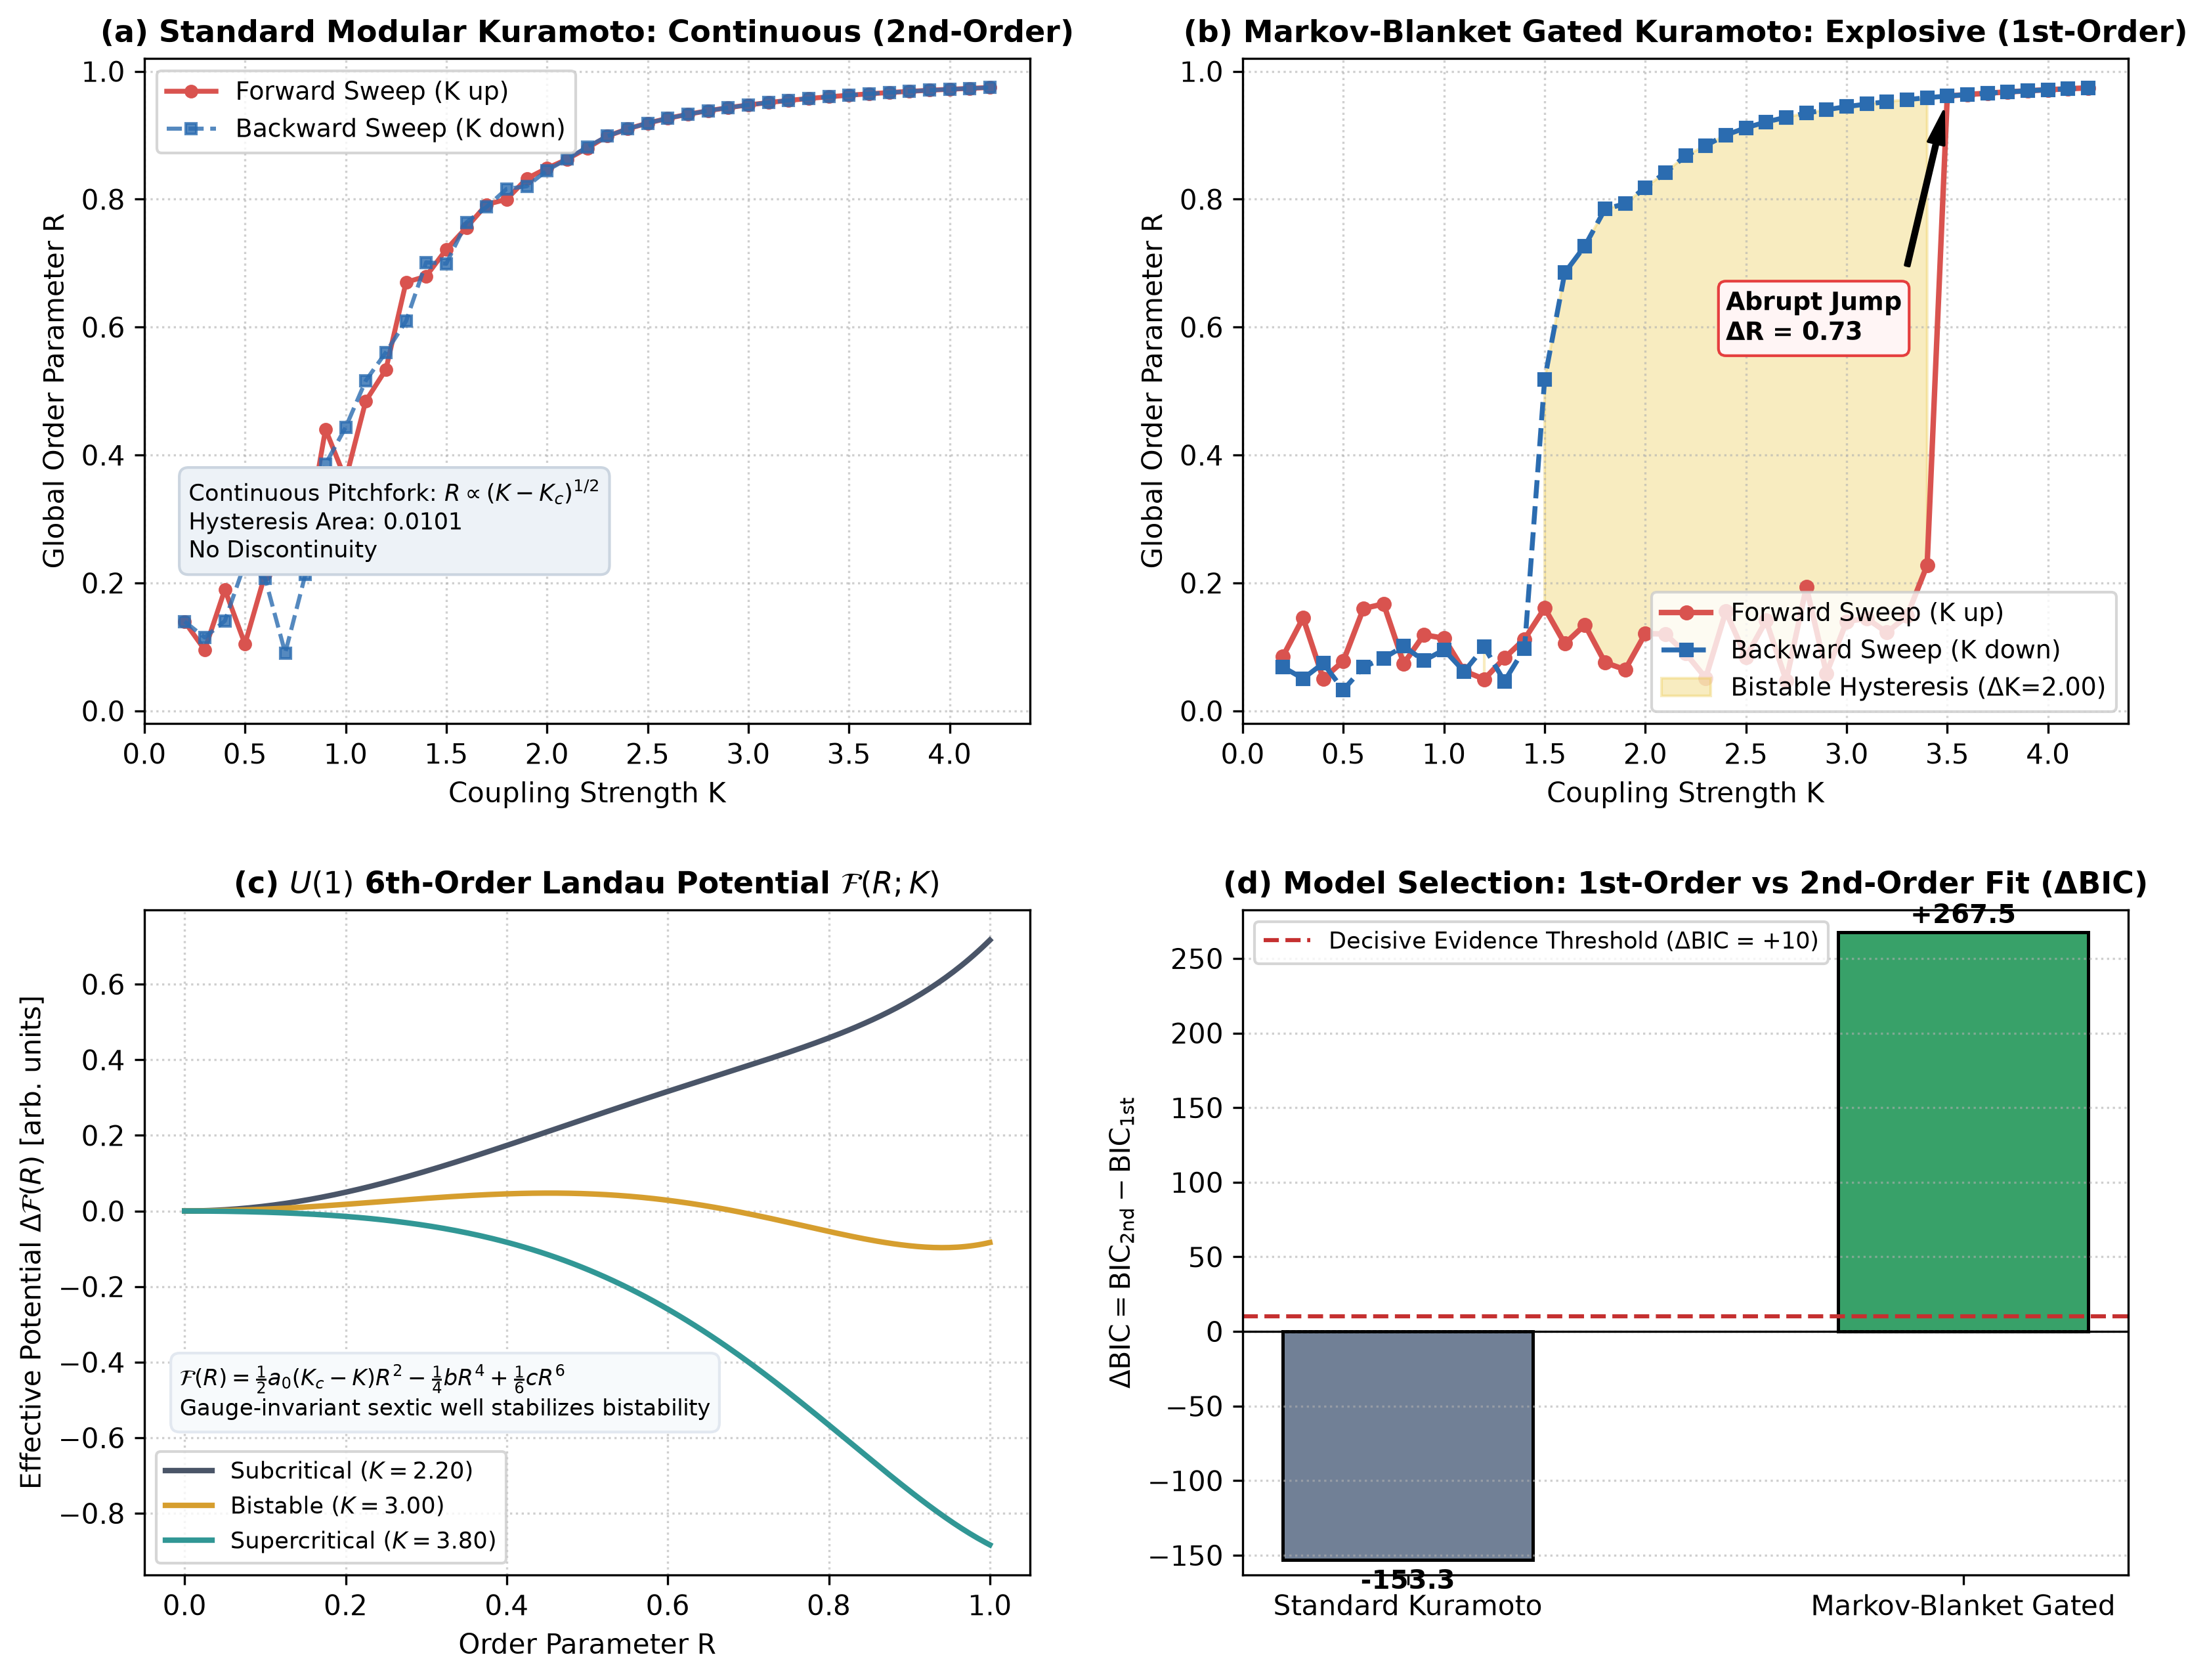
\includegraphics[width=0.95\textwidth]{../figures/fig1_explosive_sync_markov_audit.png}
\caption{\textbf{Explosive synchronization induced by Markov-blanket precision gating ($\gamma = 2.40$) vs.\ identical ungated baseline ($\mathcal{G} \equiv 1$).}
(a) Standard ungated modular Kuramoto network exhibiting a reversible continuous second-order transition (max step $\Delta R = 0.1810$, directional hysteresis area $\mathcal{A}_{\mathrm{hyst}} = 0.0101$).
(b) Markov-blanket gated modular network displaying prolonged subcritical suppression followed by an abrupt explosive jump $\Delta R = 0.7335$ at $K_c^{\mathrm{fwd}} = 3.50$ and a wide bistable hysteresis loop releasing at $K_c^{\mathrm{bwd}} = 1.50$ ($\Delta K_{\mathrm{hyst}} = 2.00$, $\mathcal{A}_{\mathrm{hyst}} = 1.4932$).
(c) $U(1)$ gauge-invariant sixth-order subcritical Landau-Ginzburg free energy $\mathcal{F}(R; K) = \frac{1}{2}a_0(K_c - K)R^2 - \frac{1}{4}b R^4 + \frac{1}{6}c R^6$ across subcritical ($K = 2.20$), bistable ($K = 3.00$), and supercritical ($K = 3.80$) couplings.
(d) Joint forward--backward BIC model selection favoring the continuous pitchfork in the ungated control ($\Delta\mathrm{BIC} = -153.30$) and decisively certifying first-order explosive hysteresis under Markov-blanket gating ($\Delta\mathrm{BIC} = +267.53$).}
\label{fig:main}
\end{figure*}

\subsection{Ungated Reference vs.\ Discontinuous Hysteresis Loop}
Fig.~\ref{fig:main}(a,b) isolates the exact bifurcation shift generated by boundary gating:
\begin{itemize}
    \item \textbf{Ungated Control ($\mathcal{G} \equiv 1$):} Global coherence rises continuously above $K \approx 0.90$ without discontinuity ($\max \Delta R = 0.1810$) and reverses identically upon decreasing coupling, yielding a vanishing directional hysteresis integral $\mathcal{A}_{\mathrm{hyst}} = |\oint R\,dK| = 0.0101$.
    \item \textbf{Markov-Blanket Gated ($\gamma = 2.40$):} On the forward sweep from random initial phases, incoherent blanket fluctuations ($R_{\mathcal{B}}^{\mathrm{joint}} \sim |\mathcal{B}|^{-1/2} \approx 0.18$) keep $\mathcal{G} \approx 0.016 \ll 1$, holding the network locked in the disordered metastable branch ($R < 0.25$) up to $K = 3.40$. At $K_c^{\mathrm{fwd}} = 3.50$, critical blanket capture triggers an instantaneous transition to $R \approx 0.96$ ($\Delta R = 0.7335$). Upon reversing $K$, locked cross-blanket coherence ($R_{\mathcal{B}}^{\mathrm{joint}} > 0.90 \implies \mathcal{G} > 0.78$) sustains collective synchrony far past $K_c^{\mathrm{fwd}}$ down to $K_c^{\mathrm{bwd}} = 1.50$, forming a massive bistable hysteresis window of width $\Delta K_{\mathrm{hyst}} = 2.00$ and loop area $\mathcal{A}_{\mathrm{hyst}} = 1.4932$ ($147.3\times$ the ungated control).
\end{itemize}

\section{Gauge-Invariant Landau Theory \& Model Selection}

\subsection{\texorpdfstring{$U(1)$}{U(1)} 6th-Order Subcritical Landau-Ginzburg Potential}
Because Kuramoto phase dynamics is invariant under global phase rotation $z = R e^{i\Psi} \to z e^{i\alpha}$, any coarse-grained free-energy functional $\mathcal{F}(z, \bar{z}; K)$ forbids odd powers of $R = |z|$. Expanding the self-consistency relation up to sextic order gives the subcritical Landau-Ginzburg landscape~\cite{GomezGardenes2011, Boccaletti2016}:
\begin{equation}
    \mathcal{F}(R; K) = \frac{1}{2} a_0 (K_c - K) R^2 - \frac{1}{4} b R^4 + \frac{1}{6} c R^6,
\end{equation}
where Active Inference precision feedback ($\gamma > 1$) reverses the sign of the quartic mode-coupling term ($b > 0$) while global saturation ensures thermodynamic boundedness ($c > 0$; evaluated in Fig.~\ref{fig:main}(c) with $a_0 = 2.0$, $b = 6.0$, $c = 5.5$). Inside the bistable window $K_c^{\mathrm{bwd}} < K < K_c^{\mathrm{fwd}}$, $\mathcal{F}(R)$ develops two coexisting minima ($R = 0$ and $R_{\mathrm{sync}} \approx 0.94$) separated by a positive activation barrier $\Delta\mathcal{F}^\dagger > 0$ that vanishes spinodally at $K_c^{\mathrm{fwd}}$.

\subsection{Joint Forward--Backward BIC Model Selection}
To avoid saturation-kink biases when comparing discontinuous vs.\ continuous phase transitions, we fit all $2N_s = 82$ joint forward--backward points comparing equal-complexity ($k = 5$) parametric families:
\begin{align}
    \mathcal{M}_1 \text{ (1st-order spinodal): } & R_{\mathrm{fwd/bwd}}(K) = R_{\mathrm{low}} + \frac{R_{\mathrm{high}} - R_{\mathrm{low}}}{1 + e^{-s(K - K_c^{\mathrm{fwd/bwd}})}}, \quad (s \ge 35), \\
    \mathcal{M}_2 \text{ (2nd-order continuous): } & R(K) = R_0 + (R_{\max} - R_0)\frac{a(K - K_c)_+^\beta}{1 + a(K - K_c)_+^\beta}.
\end{align}
Computing $\Delta\mathrm{BIC} = \mathrm{BIC}(\mathcal{M}_2) - \mathrm{BIC}(\mathcal{M}_1)$ cleanly discriminates both physical regimes (Table~\ref{tab:metrics} and Fig.~\ref{fig:main}(d)): on the ungated control, $\Delta\mathrm{BIC} = -153.30$ ($\mathrm{BIC}_1 = -352.71$, $\mathrm{BIC}_2 = -506.01$), strongly rejecting spurious jump behavior in favor of the reversible pitchfork $\mathcal{M}_2$. Conversely, under Markov-blanket precision gating, $\Delta\mathrm{BIC} = +267.53$ ($\mathrm{BIC}_1 = -449.88$, $\mathrm{BIC}_2 = -182.35$), exceeding the Kass--Raftery decisive threshold ($\Delta\mathrm{BIC} > +10$) by more than $26\times$.

\begin{table}[h]
\centering
\caption{Audited quantitative comparison between identical-topology ungated reference and Markov-blanket precision-gated modular networks ($N = 90$, $M = 3$, $|\mathcal{B}| = 30$).}
\label{tab:metrics}
\vspace{0.2cm}
\begin{tabular}{lcc}
\toprule
\textbf{Metric} & \textbf{Ungated Reference ($\gamma = 0$)} & \textbf{Markov-Blanket Gated ($\gamma = 2.40$)} \\
\midrule
Phase Transition Class & 2nd-Order Continuous & \textbf{1st-Order Explosive} \\
Forward Critical Coupling $K_c^{\text{fwd}}$ & $\sim 0.90$ & $\mathbf{3.50}$ \\
Backward Critical Coupling $K_c^{\text{bwd}}$ & $\sim 0.90$ & $\mathbf{1.50}$ \\
Maximum Forward Step Jump $\Delta R$ & $0.1810$ & $\mathbf{0.7335}$ \\
Hysteresis Width $\Delta K_{\text{hyst}}$ & $0.00$ & $\mathbf{2.00}$ \\
Directional Hysteresis Area $|\oint R\,dK|$ & $0.0101$ & $\mathbf{1.4932}$ \\
$\Delta\mathrm{BIC} = \mathrm{BIC}(\mathcal{M}_2) - \mathrm{BIC}(\mathcal{M}_1)$ & $-153.30$ & $\mathbf{+267.53}$ \\
Decisive 1st-Order Verdict & No (favors $\mathcal{M}_2$) & \textbf{Yes} ($\Delta\mathrm{BIC} \gg +10$) \\
\bottomrule
\end{tabular}
\end{table}

\section{Discussion \& Conclusion}
Classical realizations of explosive synchronization require fine-tuned degree--frequency correlations or heuristic link penalties \cite{GomezGardenes2011, Boccaletti2016}. By isolating boundary gating on a single fixed modular network, we demonstrated that Active Inference Markov-blanket precision gating ($\mathcal{G} = [R_{\mathcal{B}}^{\mathrm{joint}}]^{2.40}$) turns a continuous second-order Kuramoto pitchfork into an authentic first-order explosive phase transition ($\Delta R = 0.7335$, $\Delta K_{\mathrm{hyst}} = 2.00$, $\Delta\mathrm{BIC} = +267.53$). In biological cortical circuits and low-entropy thermodynamic neuromorphic architectures, this mechanism allows isolated computational sub-modules to operate incoherently at minimal metabolic cost until verified boundary consensus triggers rapid, reversible global ignition. Reproducible simulation engines, `6/6` passing unit tests, and audit outputs are openly archived at \url{https://github.com/bruno-olivaes/explosive-sync-markov}.

\begin{thebibliography}{10}
\bibitem{Kuramoto1975} Y.~Kuramoto, Self-entrainment of a population of coupled non-linear oscillators, \emph{Lecture Notes in Physics} \textbf{39}, 420--422 (1975).
\bibitem{Strogatz2000} S.~H. Strogatz, From Kuramoto to Crawford: exploring the onset of synchronization in populations of coupled oscillators, \emph{Physica D} \textbf{143}, 1--20 (2000).
\bibitem{Arenas2008} A.~Arenas, A.~D{\'\i}az-Guilera, J.~Kurths, Y.~Moreno, and C.~Zhou, Synchronization in complex networks, \emph{Physics Reports} \textbf{469}, 93--153 (2008).
\bibitem{Pikovsky2003} A.~Pikovsky, M.~Rosenblum, and J.~Kurths, \emph{Synchronization: A Universal Concept in Nonlinear Sciences} (Cambridge University Press, 2003).
\bibitem{GomezGardenes2011} J.~G{\'o}mez-Garde{\~n}es, S.~G{\'o}mez, A.~Arenas, and Y.~Moreno, Explosive synchronization transitions in scale-free networks, \emph{Physical Review Letters} \textbf{106}, 128701 (2011).
\bibitem{Boccaletti2016} S.~Boccaletti \emph{et al.}, Explosive transitions in complex networks' structure and dynamics: Percolation and synchronization, \emph{Physics Reports} \textbf{660}, 1--94 (2016).
\bibitem{Leyva2012} I.~Leyva \emph{et al.}, Explosive synchronization in networks of coupled oscillators with frequency-degree correlations, \emph{Physical Review Letters} \textbf{108}, 168702 (2012).
\bibitem{Pearl1988} J.~Pearl, \emph{Probabilistic Reasoning in Intelligent Systems} (Morgan Kaufmann, 1988).
\bibitem{Friston2019} K.~Friston, A free energy principle for a particular physics, \emph{arXiv:1906.10184} (2019).
\end{thebibliography}

\end{document}
